\section{60 - MAT - AG 2.1, FA 2.2 - Einkommensteuer - Matura 2015/16 Haupttermin}

\begin{langesbeispiel} \item[0] %PUNKTE DES BEISPIELS
	
 Erwerbstätige Personen müssen einen Teil ihrer Einkünfte in Form von Einkommensteuer an den Staat abführen. Im Steuermodell für das Kalenderjahr 2015 unterscheidet man vier Steuerklassen mit den sogenannten Steuersätzen: 0\,\%, 36,5\,\%, 43,2\,\% und 50\,\%. 

Modellhaft wird angenommen:  

Jahresnettoeinkommen = steuerpflichtiges Jahreseinkommen - Einkommensteuer 

Die Berechnung der Einkommensteuer bezieht sich auf das steuerpflichtige Jahreseinkommen und unterliegt für das Kalenderjahr 2015 den folgenden Regeln:
\begin{itemize}
	\item Einkommen bzw. Einkommensteile bis \EUR{11.000} sind steuerfrei.
	\item  Einkommensteile über \EUR{11.000} bis \EUR{25.000} werden mit 36,5\,\% besteuert. Das heißt: Liegt das Einkommen über \EUR{11.000}, sind die ersten verdienten \EUR{11.000} steuerfrei, die darüber hinausgehenden Einkommensteile bis \EUR{25.000} werden mit 36,5\,\% besteuert. 
	\item Einkommensteile über \EUR{25.000} bis \EUR{60.000} werden mit 43,2\,\% (genau: $43\frac{3}{14}\,\%$) besteuert. 
	\item Einkommensteile über \EUR{60.000} werden mit 50\,\% besteuert.
\end{itemize}

Am 7. Juli 2015 wurde vom Nationalrat das Steuerreformgesetz 2015/2016 beschlossen. Das ab dem 1. Jänner 2016 gültige Steuermodell ist ein Modell mit sieben Steuersätzen. Das 2015 gültige Modell (mit vier Steuerklassen) und das ab 2016 gültige Modell (mit sieben Steuerklassen) sind in der nachstehenden Grafik dargestellt.

\begin{center}
	\resizebox{1\linewidth}{!}{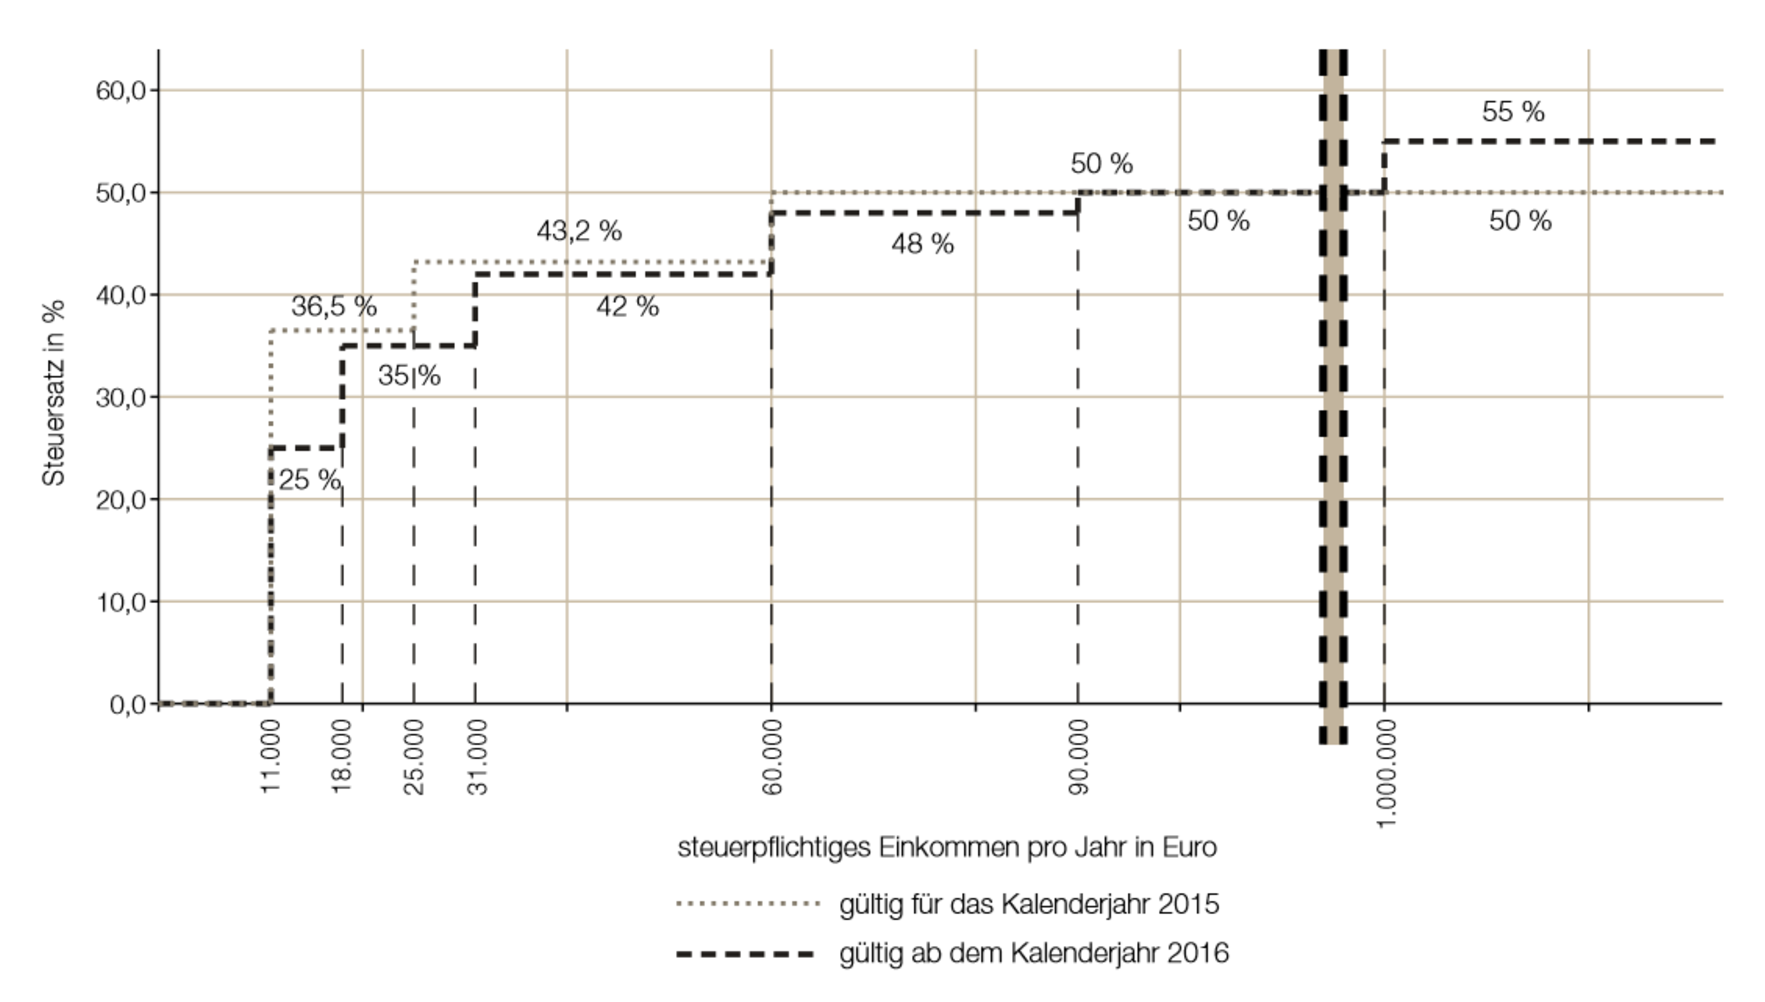
\includegraphics{../_database/Bilder/Bild60-1.eps}}
\end{center}
\begin{tiny}\begin{singlespace}  Datenquelle:  http://www.parlament.gv.at/ZUSD/BUDGET/BD\_-\_Steuerreform\_2015\_und\_2016.pdf, S. 15 [11.11.2015]\end{singlespace}\end{tiny}


\subsection{Aufgabenstellung:}
\begin{enumerate}
	\item \fbox{A} Berechne mithilfe der 2015 geltenden Steuersätze das Jahresnettoeinkommen einer Person, deren steuerpflichtiges Jahreseinkommen \EUR{20.000} beträgt!
	
	Gib (für das Jahr 2015) eine Formel für das Jahresnettoeinkommen $N$ einer Person an, deren steuerpflichtiges Jahreseinkommen $E$ zwischen \EUR{11.000} und \EUR{25.000} liegt!
	
	\item Der sogenannte \textit{Durchschnittssteuersatz} ist wie folgt definiert:
	
	$\text{Durchschnittssteuersatz}=\frac{\text{gezahlte Einkommensteuer}}{\text{steuerpflichtiges Jahreseinkommen}}$
	
	Jemand bezog im Jahr 2015 ein steuerpflichtiges Jahreseinkommen von \EUR{40.000}. Berechne für diese Person für das Jahr 2015 den Durchschnittssteuersatz! 
 
Interpretiere unter Verwendung der gegebenen Grafik, was für diese Person mit dem Term $7\,000\cdot 0,115+7\,000\cdot 0,015+6\,000\cdot 0,082+9\,000\cdot 0,012$ berechnet wird!

\item Jemand behauptet:
\begin{enumerate}
	\item "`Bei einem steuerpflichtigen Jahreseinkommen von \EUR{100.000} tritt trotz der Gesetzesänderung keine Veränderung hinsichtlich der abzuführenden Einkommensteuer ein."'
	
	\item "`Der Steuersatz für steuerpflichtige Jahreseinkommen von über \EUR{11.000} bis \EUR{18.000} ändert sich um 11,5 Prozent."'
\end{enumerate}
	
	Sind diese Behauptungen richtig? Formuliere jeweils eine mathematisch begründete Antwort!
	
	\item Das Bundesministerium für Finanzen gibt auf seiner Website die Berechnung der Einkommensteuer 2015 (ESt) für die Einkommensklasse über \EUR{25.000} bis \EUR{60.000} steuerpflichtiger Jahreseinkommen mit folgender Formel an:\leer
	
	$\text{ESt}=\frac{(\text{steuerpflichtiges Jahreseinkommen}-25\,000)\cdot 15\,125}{35\,000}+5\,110$\leer
	
	Deute den Faktor $\frac{15\,125}{35\,000}$ und den Summanden $5\,110$ im Hinblick auf die Berechnung der Einkommensteuer!\leer
	
	Stelle eine Formel zur Berechnung der Einkommensteuer $(\text{ESt}_\text{neu})$ für ein steuerpflichtiges Jahreseinkommen von über \EUR{31.000} bis \EUR{60.000} für das ab 2016 gültige Steuermodell auf!\leer
	
	$(\text{ESt}_\text{neu})$= \rule{5cm}{0.3pt}

						\end{enumerate}\leer
				
\antwort{
\begin{enumerate}
	\item \subsection{Lösungserwartung:} 
	
$20\,000-9\,000\cdot 0,365=16\,715 \Rightarrow$ \EUR{16.715}\leer

Mögliche Formeln:

$N=E-(E-11\,000)\cdot 0,365$

oder:

$N=11\,000+(E-11\,000)\cdot 0,635$

	\subsection{Lösungsschlüssel:}
	\begin{itemize}
		\item Ein Ausgleichspunkt für die richtige Lösung, wobei die Einheit "`\EUR{}"' nicht angegeben sein muss. 
		
		Toleranzintervall: [\EUR{16.700}; \EUR{16.720}] 
		\item Ein Punkt für die Angabe einer korrekten Formel für das Jahresnettoeinkommen. Äquivalente Formeln sind als richtig zu werten.
	\end{itemize}
	
	\item \subsection{Lösungserwartung:}
			
	$\frac{14\,000\cdot 0,365+15\,000\cdot 0,432}{40\,000}\approx 0,29,$ d.h. ca. $29\,\%$ Durschnittssteuersatz
	
	Mit dem Term wird die Steuerersparnis (in Euro) dieser Person durch das neue Steuermodell (im Vergleich zum 2015 gültigen Modell) berechnet.

	\subsection{Lösungsschlüssel:}
	
\begin{itemize}
	\item Ein Punkt für die richtige Lösung.
	
	Toleranzintervall: $[0,28;0,29]$ bzw. $[28\,\%; 29\,\%]$
	\item   Ein Punkt für eine (sinngemäß) richtige Interpretation.
\end{itemize}

\item \subsection{Lösungserwartung:}
			
Beide Behauptungen sind falsch.

\begin{enumerate}
	\item Auch  Bezieher/innen von einem steuerpflichtigen Jahreseinkommen von \EUR{100.000} bezahlen beim neuen Steuermodell weniger Einkommensteuer, nämlich für die Einkommensanteile unter \EUR{90.000}. 
	\item Tatsächlich ändert sich der Steuersatz für das steuerpflichtige Jahreseinkommen um 11,5 \textit{Prozentpunkte}, das sind $\frac{11,5}{36,5}\approx 31,5$ \textit{Prozent}.
\end{enumerate}

	\subsection{Lösungsschlüssel:}
	
\begin{itemize}
	\item Ein Punkt für eine (sinngemäß) richtige Begründung, warum die Behauptung (i) falsch ist.
	\item Ein Punkt für eine (sinngemäß) richtige Begründung, warum die Behauptung (ii) falsch ist.
\end{itemize}

\item \subsection{Lösungserwartung:}
			
$\frac{15\,125}{35\,000}\approx 0,432$ ist der Steuersatz für diese Einkommensklasse.

5\,110 ist die Einkommensteuer für die ersten \EUR{25.000} an steuerpflichtigem Jahreseinkommen.

$\text{ESt}_\text{neu}=(\text{steuerpflichtiges Jahreseinkommen}-31\,000)\cdot 0,42+6\,300$
	\subsection{Lösungsschlüssel:}
	
\begin{itemize}
	\item Ein Punkt für eine (sinngemäß) richtige Interpretation beider Zahlenwerte.
	\item Ein Punkt für eine korrekte Formel. Äquivalente Formeln sind als richtig zu werten.
\end{itemize}

\end{enumerate}}
		\end{langesbeispiel}